% Paper para CACIC 2026 --- ENVÍO CIEGO.
% No agregar autores, afiliaciones, agradecimientos, financiamiento, URL del
% repositorio ni ORCID. Verificar con:
%     python scripts/check_anonimato.py paper/02_reescrito
\documentclass[runningheads]{llncs}
\usepackage[T1]{fontenc}
\usepackage[utf8]{inputenc}
\usepackage[spanish,es-tabla,es-noquoting]{babel}
\usepackage{graphicx}
\usepackage{booktabs}
% NOTA DE IMPLEMENTACION (subtask 14): llncs.cls de "LaTeX2e (1)/" NO carga
% hyperref pese a lo asumido en el plan ("que llncs ya carga"); sin este
% \usepackage, \hypersetup produce "Undefined control sequence" y no hay
% forma de forzar vacios los metadatos del PDF (requisito de envio ciego).
\usepackage{hyperref}

\hypersetup{pdfauthor={},pdfsubject={},pdfkeywords={}}

\begin{document}

\title{Modelos de Lenguaje Pequeños para la Interpretación de Comandos de
Domótica en Español: Evaluación Automática de Doce Modelos Sub-2B}
\titlerunning{SLMs para Comandos de Domótica en Español}
\author{Anonimizado por revisión ciega}
\authorrunning{Anonimizado por revisión ciega}
\institute{Anonimizado por revisión ciega}
\maketitle

\begin{abstract}
Los asistentes de domótica basados en modelos de lenguaje suelen depender de
servicios en la nube, lo que introduce alta latencia, costos recurrentes y
dependencia de conectividad. Los Small Language Models (SLMs) ejecutados
localmente constituyen una alternativa viable para hubs domóticos de bajo
costo, pero su capacidad para interpretar comandos en español rioplatense no
ha sido evaluada: el voseo, los diminutivos y las expresiones relativas de la
variedad (``bajale un toque'') no aparecen en los corpus de domótica en
inglés usados para entrenar y evaluar estos modelos, y su tratamiento no
puede suponerse transferido. Este trabajo evalúa doce SLMs abiertos de menos
de 2 mil millones de parámetros sobre un dataset de 32 comandos en español
rioplatense, con anotación de referencia de cinco campos (intención,
dispositivo, ubicación, valor y unidad). La verificación es automática en dos
etapas: comparación textual determinista campo a campo y un modelo de
lenguaje que actúa de juez, clasificando cada respuesta incorrecta contra una
taxonomía cerrada. Se reportan exactitud estricta y exactitud laxa
(semántica): su brecha cuantifica cuánto penaliza la coincidencia textual
exacta a respuestas que un evaluador humano consideraría correctas.

\keywords{modelos de lenguaje pequeños, domótica, evaluación automática,
LLM como juez, procesamiento del lenguaje natural, español rioplatense.}
\end{abstract}

\section{Introducción}

El crecimiento de los asistentes de voz y los sistemas domóticos ha
popularizado el uso de modelos de lenguaje para interpretar comandos en
lenguaje natural (``prendé la luz del living'', ``bajá el aire a 20
grados''). La mayoría de las soluciones comerciales dependen de modelos de
gran escala alojados en la nube, lo que introduce tres problemas recurrentes
en el contexto de un hogar: latencia de red, costo recurrente por uso de
API, y dependencia de conectividad — un comando tan simple como apagar una
luz no debería fallar por una caída de internet.

Una alternativa creciente es el uso de Small Language Models (SLMs) —
modelos de lenguaje de entre unos cientos de millones y pocos miles de
millones de parámetros — ejecutados localmente en el propio hub domótico
(una Raspberry Pi, un mini-PC o un microcontrolador de gama alta). Trabajos
recientes muestran que estos modelos pueden alcanzar, en tareas acotadas, un
desempeño competitivo frente a modelos mucho más grandes \cite{gupta2025slms}.
Sin embargo, la mayor parte de la literatura sobre SLMs y asistentes
domóticos evalúa el inglés, y no está claro cómo se comportan estos modelos
frente a estructuras propias del español rioplatense (voseo, diminutivos,
expresiones relativas como ``bajale un toque'') ni cuál es el costo real en
latencia de ejecutarlos en hardware modesto.

La clasificación manual de respuestas incorrectas para identificar patrones
de error no escala a un roster de doce modelos: multiplica el volumen de
respuestas a revisar a mano, y su resultado tampoco es reproducible por un
tercero, porque depende del criterio del anotador en el momento de
clasificar cada caso. Este trabajo evalúa doce SLMs mediante un pipeline de
verificación completamente automático, sobre un roster que incorpora
familias de modelos publicadas recientemente (LFM2.5, Granite 4.0, Qwen3.5
y OLMo-2) junto con dos tiers de tamaño (menos de 1000 millones y entre
1000 y 2000 millones de parámetros).

Las contribuciones de este trabajo son: (1) la evaluación de un roster de
doce modelos abiertos sub-2B, de acceso público y sin restricción de
licencia ni de token de acceso, organizados en dos tiers de tamaño de seis
modelos cada uno y evaluados bajo un protocolo común; (2) un pipeline de
verificación automática en dos etapas, coincidencia textual determinista
más un juez de lenguaje con una taxonomía cerrada, que elimina el
etiquetado manual de respuestas incorrectas y de categorías lingüísticas;
(3) el reporte conjunto de exactitud estricta y exactitud laxa, cuya
brecha cuantifica el costo de exigir coincidencia textual exacta; (4) un
protocolo de ejecución reproducible, con aislamiento por contenedor y
versiones de librerías documentadas por grupo; y (5) la inclusión
deliberada de un modelo representativo de la generación anterior de SLMs
(\texttt{Qwen2.5-1.5B-Instruct}), evaluado bajo el mismo protocolo que el
resto del roster, que permite cuantificar cuánto cambió lo factible para
esta tarea en el rango sub-2B respecto de esa generación.

\section{Trabajos relacionados}

Convertir un comando en una estructura de intención y argumentos (slots) es
una tarea clásica de Natural Language Understanding (NLU). Weld et al.
\cite{weld2023survey} relevan los modelos conjuntos de detección de intención
y slot filling previos a los grandes modelos de lenguaje (LLMs), entrenados
específicamente para el dominio; son el punto de comparación natural del
enfoque actual, que resuelve la misma tarea generando directamente un JSON
con un modelo general. Bouraoui et al. \cite{bouraoui2018french} mostraron,
sobre un corpus de comandos de voz para hogar inteligente en francés, que los
recursos de NLU en inglés no transfieren bien a otras lenguas y que cada
idioma requiere corpus propios; este trabajo sigue esa lógica para el español
rioplatense, con un dataset de evaluación y no de entrenamiento.

El antecedente más cercano evalúa LLMs on-device para home assistants
\cite{ondevice2025homeassistant}: variantes cuantizadas de 16, 8 y 4 bits en
el doble rol de detección de intención y generación de respuesta, con
80\%--86\% de exactitud y latencias de 5 a 6 segundos. Este trabajo se
diferencia en el extremo inferior de tamaño (sub-2B, sin cuantización
agresiva), el idioma, y la interpretación estructurada en lugar de la
generación conversacional. El survey de Lu et al. \cite{gupta2025slms}
documenta que modelos de pocos miles de millones de parámetros alcanzan
paridad de tarea específica frente a modelos mucho mayores cuando se entrenan
con datos de alta calidad; los reportes técnicos de Qwen2.5
\cite{qwen2024report}, SmolLM2 \cite{allal2024smollm2} y OLMo 2
\cite{olmo2report} describen tres de las familias evaluadas aquí.

La decodificación restringida por gramática garantiza validez sintáctica con
independencia de la capacidad del modelo
\cite{beurerkellner2024guiding,dong2024xgrammar}. Este estudio optó
deliberadamente por no usarla, para medir el seguimiento de instrucciones en
un despliegue simple: resuelve la validez de formato, pero no evita que el
modelo alucine un valor semánticamente incorrecto dentro de un JSON válido,
patrón que la taxonomía de la Sección \ref{sec:dos-etapas} distingue.

La técnica central que este trabajo incorpora es la evaluación con un modelo
de lenguaje como juez. Zheng et al. \cite{zheng2023judging} muestran que un
LLM suficientemente capaz aproxima el juicio humano con acuerdo alto, y
proponen la técnica donde la coincidencia exacta subestima el desempeño real
— el caso de este trabajo, donde un sinónimo válido de un dispositivo no
coincide con el ground truth. Su limitación conocida es el sesgo de
auto-favorecimiento; como aquí el juez es uno de los modelos evaluados,
aplica directamente y se retoma en la Sección 6.

\section{Metodología}

\subsection{Modelos evaluados}

\begin{table}[htbp]
\centering
\caption{Conjunto de modelos evaluados, con la versión de \texttt{transformers} resuelta para cada uno. La línea horizontal separa la franja sub-1B (arriba) de la franja 1--2B (abajo). Forzaron el pin: tokenizer no soportado en 4.57.6 (\texttt{LFM2.5-230M}); íd. (mismo tokenizer) (\texttt{LFM2.5-350M}); regresión de caché en la versión 5.14.1 (\texttt{granite-4.0-350m}); arquitectura no reconocida en 4.57.6 (\texttt{Qwen3.5-0.8B}).}
\label{tab:modelos}
{\footnotesize
\begin{tabular}{lrlr}
\toprule
Modelo & Parámetros & Familia & \texttt{transformers} \\
\midrule
LFM2.5-230M & 0.23B & LiquidAI & 5.14.1 \\
granite-4.0-h-350m & 0.34B & IBM Granite & 4.57.6 \\
LFM2.5-350M & 0.35B & LiquidAI & 5.14.1 \\
granite-4.0-350m & 0.35B & IBM Granite & 4.57.6 \\
SmolLM2-360M-Instruct & 0.36B & HuggingFaceTB & 4.57.6 \\
Qwen3.5-0.8B & 0.80B & Qwen & 5.14.1 \\
\midrule
OLMo-2-0425-1B-Instruct & 1.00B & AllenAI & 4.57.6 \\
LFM2.5-1.2B-Instruct & 1.20B & LiquidAI & 4.57.6 \\
granite-4.0-h-1b & 1.50B & IBM Granite & 4.57.6 \\
Qwen2.5-1.5B-Instruct & 1.54B & Qwen & 4.57.6 \\
granite-4.0-1b & 1.60B & IBM Granite & 4.57.6 \\
SmolLM2-1.7B-Instruct & 1.71B & HuggingFaceTB & 4.57.6 \\
\bottomrule
\end{tabular}
}
\end{table}


Se evaluaron doce modelos abiertos, públicos en HuggingFace y sin
restricción de licencia ni de token, en dos franjas de seis: sub-1B y de 1
a 2B (Tabla
\ref{tab:modelos}). \texttt{Qwen2.5-1.5B-Instruct} (1,54\,B) se incorporó
deliberadamente como representante de la generación anterior de SLMs bajo el
mismo protocolo (Sección \ref{sec:resultados-globales}).

\subsection{Dataset de comandos}

El dataset consta de 32 comandos de domótica en español rioplatense (voseo),
con una anotación de referencia de cinco campos: \texttt{intent},
\texttt{dispositivo}, \texttt{ubicacion}, \texttt{valor} y \texttt{unidad}.
Cada comando pertenece además a una de seis categorías lingüísticas cerradas
— encendido/apagado simple, ajuste con valor numérico explícito, ajuste
relativo o cualitativo, múltiples dispositivos, consulta de estado y negación
o contexto conversacional —, que asigna el juez automático (Sección
\ref{sec:dos-etapas}) y no un anotador humano.

\subsection{Protocolo de prompting y esquema de salida}
\label{sec:prompting}

El prompt de sistema es único y fijo para los doce modelos, aplicado
mediante la plantilla de conversación del propio \emph{tokenizer} de cada
uno. Se transcribe íntegro junto con el prompt de usuario; ambos provienen
de constantes del código, no de una transcripción manual.

\paragraph{Prompt de sistema (texto completo).}
{\footnotesize\ttfamily
\begin{verbatim}
Sos un módulo de interpretación de comandos de voz para un sistema
domótico en español rioplatense. Convertí el comando del usuario en UN
objeto JSON con estos campos: "intent"
(encender/apagar/ajustar/consultar), "dispositivo" (luz,
aire_acondicionado, calefaccion, persiana, cortina, tv, parlante,
cerradura, ventilador, todos), "ubicacion" (living, cocina, dormitorio,
bano, garage, patio, entrada, todas), "valor" (número si el comando lo
da, si no null), "unidad" ("%" o "°C" si corresponde, si no null).
Reglas: respondé SOLO el JSON, sin texto adicional; si el comando ajusta
sin dar un número, "valor" y "unidad" deben ser null.

Ejemplo: Comando: "Poné el aire de la cocina en 20 grados."
{"intent": "ajustar", "dispositivo": "aire_acondicionado", "ubicacion":
"cocina", "valor": 20, "unidad": "°C"}

IMPORTANTE: los campos "intent", "dispositivo", "ubicacion" y "unidad"
son campos CATEGORICOS CERRADOS. Los valores listados entre parentesis
mas arriba son, textualmente, los unicos outputs aceptados para esos
campos: copialos exactamente como aparecen, sin tildes, sin mayusculas,
sin plural y sin reformular. Usar un sinonimo, una traduccion o
cualquier variante que no este literalmente en esa lista (por ejemplo
"televisor" o "tele" en lugar de "tv") es una violacion del formato y la
respuesta se considera incorrecta. Si ningun valor de la lista aplica,
usa null.

Ejemplo 2: Comando: "Bajale un poco a la luz del living."
{"intent": "ajustar", "dispositivo": "luz", "ubicacion": "living",
"valor": null, "unidad": null}
\end{verbatim}
}

\paragraph{Prompt de usuario (uno por comando, tras el de sistema).}
{\footnotesize\ttfamily
\begin{verbatim}
Comando: "<comando del usuario>"
\end{verbatim}
}


El prompt solicita un único objeto JSON con los cinco campos, incluye dos
ejemplos \emph{few-shot} y agrega una cláusula taxativa sobre los campos
categóricos cerrados: los valores listados entre paréntesis son,
textualmente, las únicas salidas aceptadas, y un sinónimo válido en español
—``tele'' por ``tv''— constituye una violación de formato. Los resultados de
la Sección \ref{sec:resultados} se calculan bajo este prompt, por lo que la comparación entre
arquitecturas nunca mezcla prompts.

\subsection{Métricas}
\label{sec:metricas}

La \textbf{exactitud estricta} exige que los cinco campos coincidan
textualmente con la referencia bajo ese protocolo taxativo; la
\textbf{exactitud laxa (semántica)} incorpora además los casos que el juez
etiquetó como \texttt{sin\_error\_semantico} o \texttt{uso\_de\_sinonimos}. La
estricta es la métrica primaria; la laxa es una cota superior que separa
errores de forma de errores de contenido, y la brecha entre ambas es un
resultado del estudio, no una corrección que deba promediarse. Se reportan
además la tasa de JSON válido, la exactitud por campo y por categoría, y la
latencia promedio.

\subsection{Verificación automática en dos etapas}
\label{sec:dos-etapas}

En la \textbf{etapa 1} cada respuesta se compara campo a campo, de forma
determinista, contra la referencia, sin ningún modelo adicional, y de ahí
sale la exactitud estricta. El juez de la \textbf{etapa 2} se determina por
una regla fijada de antemano: el modelo con mayor exactitud estricta en la
etapa 1, con empates resueltos por mayor cantidad de parámetros y luego por
el orden del listado. Ambas etapas usan decodificación \emph{greedy}
(\texttt{do\_sample=False}, temperatura 0); de eso — no de fijar el
identificador del juez de antemano — depende la reproducibilidad.

El juez clasifica cada respuesta con \texttt{match\_exact = False} en un
subconjunto no vacío de siete etiquetas cerradas — confusión de intención, de
dispositivo y de ubicación; alucinación de valor o unidad; valor numérico
incorrecto; más \texttt{sin\_error\_semantico} y \texttt{uso\_de\_sinonimos},
que definen la exactitud laxa — y asigna a cada comando exactamente una
categoría lingüística. Una salida que no valide contra ese vocabulario se
reintenta una vez y, si vuelve a fallar, recibe una etiqueta de respaldo
determinista; su frecuencia se reporta. Al ser uno de los modelos evaluados,
el juez adjudica también sobre sus propias respuestas (Sección \ref{sec:amenazas}).

\subsection{Entorno de ejecución y reproducibilidad}
\label{sec:entorno-repro}

El host es un equipo con procesador Intel Core i5-11400H (6 núcleos físicos / 12 hilos), sin GPU:
los doce modelos y el juez se ejecutan en CPU, cada uno en su propia imagen
de contenedor y de forma secuencial.

El conjunto evaluado necesita \textbf{dos grupos de versión} de
\texttt{transformers}, mutuamente excluyentes (Tabla \ref{tab:modelos}):
4.57.6 para nueve modelos y 5.14.1 para los otros tres.
\texttt{granite-4.0-350m} falla bajo 5.14.1, y \texttt{LFM2.5-230M},
\texttt{LFM2.5-350M} y \texttt{Qwen3.5-0.8B} fallan bajo 4.57.6: el segundo
grupo se resuelve precisamente a la versión que hace fallar al modelo que
impone el primero, de modo que ninguna versión mayor única cubre el conjunto
(Sección \ref{sec:amenazas}).

La configuración de Docker de esta máquina expone únicamente \textbf{dos
procesadores lógicos} y un límite de \textbf{8\,GB}, y las trece ejecuciones
— doce del barrido más la del juez — fijan \texttt{-{}-memory=8g -{}-cpus=2
-{}-cpuset-cpus=0-1}, el mismo par de identificadores lógicos en todas. Que
ese par corresponda a un mismo núcleo físico por \emph{hyperthreading} (SMT)
o a dos núcleos distintos lo decide el hipervisor y no es observable desde el
contenedor. La ejecución es secuencial porque la inferencia en CPU está
limitada por el ancho de banda de memoria, que no se particiona por
contenedor. Ninguno de estos factores afecta a la exactitud, calculada con decodificación
determinista, pero sí a las latencias: comparables entre los doce modelos,
aunque sus valores absolutos no sean los mejores alcanzables en
CPU\footnote{Código y datos: \url{https://github.com/carlosbinker/cacic-2026}
(rama \texttt{feat/reescritura-experimento-2026}).} (Sección \ref{sec:amenazas}).

\section{Experimentación y resultados}

\subsection{Resultados globales}

\begin{table}[htbp]
\centering
\caption{Resultados globales por modelo (JSON válido, exactitud estricta y laxa, latencia) y distribución de errores de la taxonomía, en las mismas doce filas. I: incorrectas; CI: confusión de intención; CD: confusión de dispositivo; CU: confusión de ubicación; VN: valor numérico incorrecto; SE: sin error semántico (equivalente por otro motivo); US: uso de sinónimos (difiere solo por un sinónimo).}
\label{tab:resultados}
{\setlength{\tabcolsep}{2pt}
{\footnotesize
\begin{tabular}{lrrrrrrrrrrr}
\toprule
Modelo & JSON & Estr. & Laxa & Lat. & I & CI & CD & CU & VN & SE & US \\
\midrule
LFM2.5-230M & 87.5 & 6.2 & 34.4 & 6.31 & 30 & 0 & 20 & 4 & 0 & 1 & 8 \\
granite-4.0-h-350m & 100.0 & 40.6 & 71.9 & 56.45 & 19 & 0 & 9 & 0 & 0 & 3 & 7 \\
LFM2.5-350M & 100.0 & 0.0 & 37.5 & 9.62 & 32 & 0 & 20 & 5 & 0 & 1 & 11 \\
granite-4.0-350m & 100.0 & 28.1 & 62.5 & 13.77 & 23 & 3 & 9 & 0 & 0 & 5 & 6 \\
SmolLM2-360M-Instruct & 25.0 & 9.4 & 93.8 & 20.47 & 29 & 0 & 2 & 0 & 0 & 1 & 26 \\
Qwen3.5-0.8B & 100.0 & 75.0 & 84.4 & 18.17 & 8 & 1 & 4 & 0 & 0 & 0 & 3 \\
OLMo-2-0425-1B-Instruct & 100.0 & 3.1 & 37.5 & 35.31 & 31 & 0 & 19 & 3 & 1 & 2 & 9 \\
LFM2.5-1.2B-Instruct & 100.0 & 56.2 & 84.4 & 31.88 & 14 & 2 & 3 & 0 & 0 & 2 & 7 \\
granite-4.0-h-1b & 100.0 & 71.9 & 96.9 & 123.14 & 9 & 0 & 1 & 0 & 0 & 7 & 1 \\
Qwen2.5-1.5B-Instruct & 100.0 & 65.6 & 93.8 & 38.13 & 11 & 0 & 1 & 1 & 0 & 2 & 7 \\
granite-4.0-1b & 100.0 & 90.6 & 100.0 & 42.78 & 3 & 0 & 0 & 0 & 0 & 1 & 2 \\
SmolLM2-1.7B-Instruct & 100.0 & 50.0 & 84.4 & 56.71 & 16 & 0 & 5 & 0 & 0 & 5 & 6 \\
\bottomrule
\end{tabular}
}
}
\end{table}


\begin{figure}[htbp]
\centering
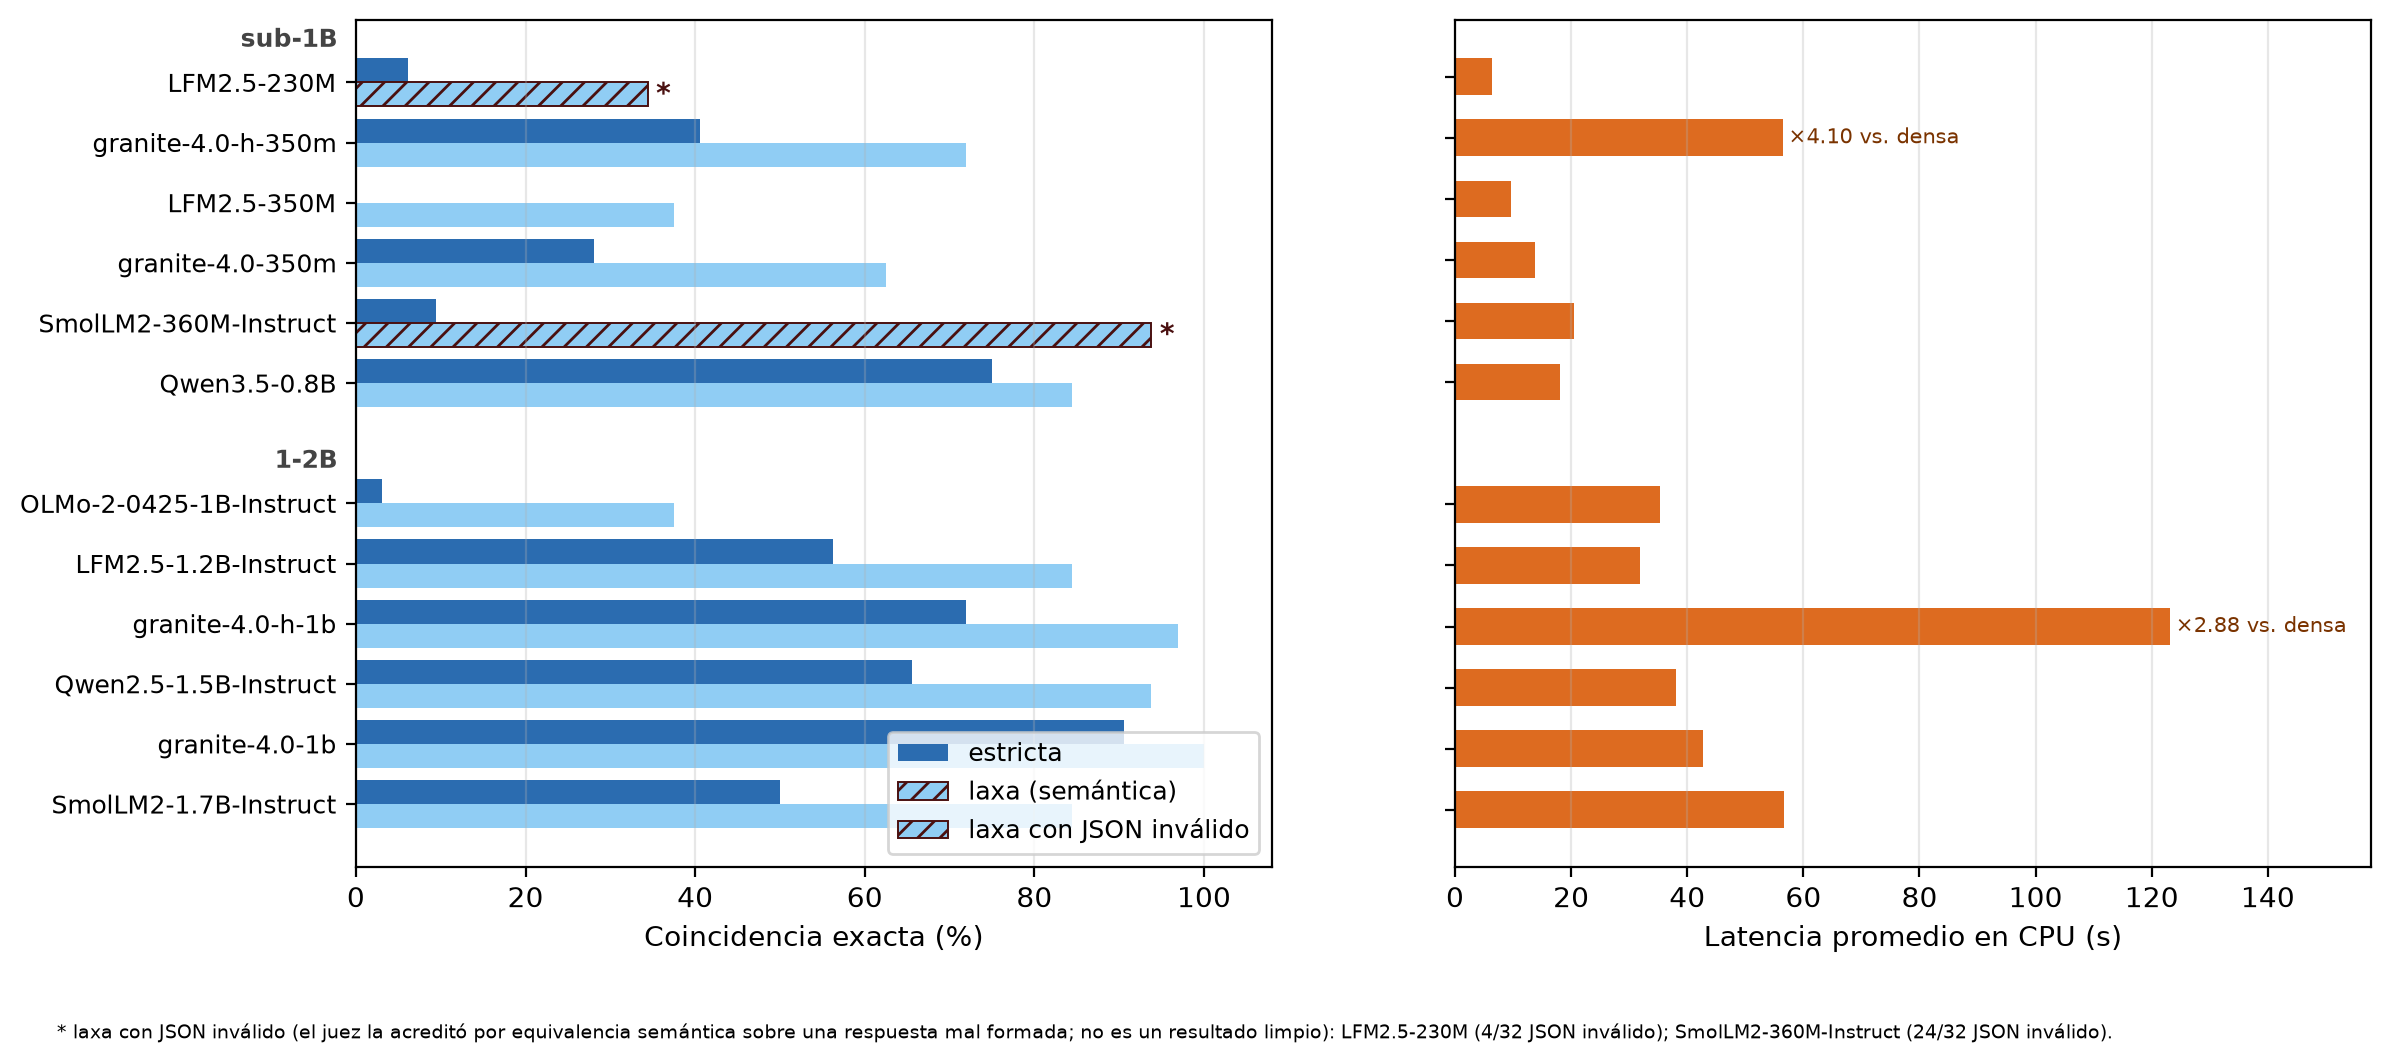
\includegraphics[width=\textwidth]{figuras/fig1_exactitud_latencia_2026.png}
\caption{Coincidencia exacta estricta y laxa (izquierda) y latencia promedio de
inferencia en CPU (derecha), por modelo, agrupados por tamaño.}
\label{fig:globales}
\end{figure}

El barrido principal se completó sobre los doce modelos del roster activo sin
ninguna falla irrecuperable: las 384 filas (12 modelos $\times$ 32 comandos) de
la Tabla \ref{tab:globales} están completas.

Bajo el prompt 2026 mantenido fijo a ambos lados de la comparación,
\texttt{granite-4.0-1b} alcanza \textbf{90,6\%} de exactitud estricta, la cifra
más alta de las doce evaluadas, frente al \textbf{65,6\%} de
\texttt{Qwen2.5-1.5B-Instruct}, el mejor modelo del brazo de generación
anterior medido idénticamente bajo ese mismo prompt: una diferencia de
\textbf{+25,0 puntos porcentuales}. En el otro extremo, \texttt{LFM2.5-350M}
no acierta ninguno de los 32 comandos bajo el protocolo estricto (0,0\%) pese a
emitir JSON válido en el 100\% de sus respuestas (Tabla \ref{tab:globales});
esa combinación se retoma en la Sección \ref{sec:analisis-errores} como fallo
semántico genuino, no como un artefacto de formato.

La ventaja del tier 1--2B sobre el tier sub-1B se sostiene en promedio, pero
no es universal: \texttt{Qwen3.5-0.8B}, el único modelo sub-1B con exactitud
estricta de tres dígitos de magnitud comparable a los mejores del tier
superior, supera en la Tabla \ref{tab:globales} a cuatro de los seis modelos
del tier 1--2B (\texttt{LFM2.5-1.2B-Instruct}, \texttt{OLMo-2-0425-1B-Instruct},
\texttt{SmolLM2-1.7B-Instruct} y \texttt{Qwen2.5-1.5B-Instruct}), y sólo queda
por debajo de las dos variantes de \texttt{granite-4.0} de mayor tamaño. Ese
desempeño, sin embargo, tiene un costo en latencia que no es uniforme dentro
del propio tier: la Sección \ref{sec:discusion-latencia-hibrida} discute en
detalle el caso de las variantes híbridas de \texttt{granite-4.0}, que
multiplican su latencia respecto de la variante densa del mismo tamaño sin
una ganancia de exactitud proporcional.

La Figura \ref{fig:globales} y la Tabla \ref{tab:globales} muestran además
que la brecha entre exactitud estricta y laxa es grande y desigual entre
modelos: en varios casos la exactitud laxa más que duplica a la estricta.
Esa brecha es, en sí misma, un resultado de este trabajo y no un simple
matiz — se retoma con el detalle por categoría de error en la Sección
\ref{sec:analisis-errores} y se discute en la Sección 5, porque parte de esa
brecha resulta poco confiable exactamente donde la validez de formato es
débil.

\textbf{Continuidad con la ronda inicial de este experimento.}
\label{sec:continuidad}
Tres de los doce modelos del roster activo —\texttt{SmolLM2-360M-Instruct},
\texttt{Qwen2.5-1.5B-Instruct} y \texttt{SmolLM2-1.7B-Instruct}— también
habían sido medidos en una ronda inicial de este mismo experimento (2025).
Para esos tres, y sólo para esos tres, la Tabla \ref{tab:globales} agrega
dos columnas de continuidad, ``Estricta 2025 (\%)'' y ``Latencia 2025 (s)'',
tomadas directamente de esa medición inicial; los otros nueve modelos
llevan un guion en esas dos columnas porque no tienen contraparte en esa
ronda. Comparando exclusivamente esas dos columnas contra las
correspondientes de este trabajo: la exactitud estricta de
\texttt{SmolLM2-360M-Instruct} desciende respecto de la medición inicial,
la de \texttt{Qwen2.5-1.5B-Instruct} sube, y la de \texttt{SmolLM2-1.7B-Instruct}
también desciende; en latencia, \texttt{SmolLM2-360M-Instruct} sube respecto
de la medición inicial mientras que \texttt{Qwen2.5-1.5B-Instruct} y
\texttt{SmolLM2-1.7B-Instruct} bajan. Ninguna de las tres cifras estrictas se
mueve en la misma dirección que las otras dos, lo que ya es un primer
indicio de que el modelo por sí solo no explica la diferencia; la
interpretación completa de este patrón, atribuido al protocolo y al arnés de
ejecución y no al modelo, se desarrolla en la Sección 5.

\subsection{Exactitud por campo del esquema}

\begin{figure}[htbp]
\centering
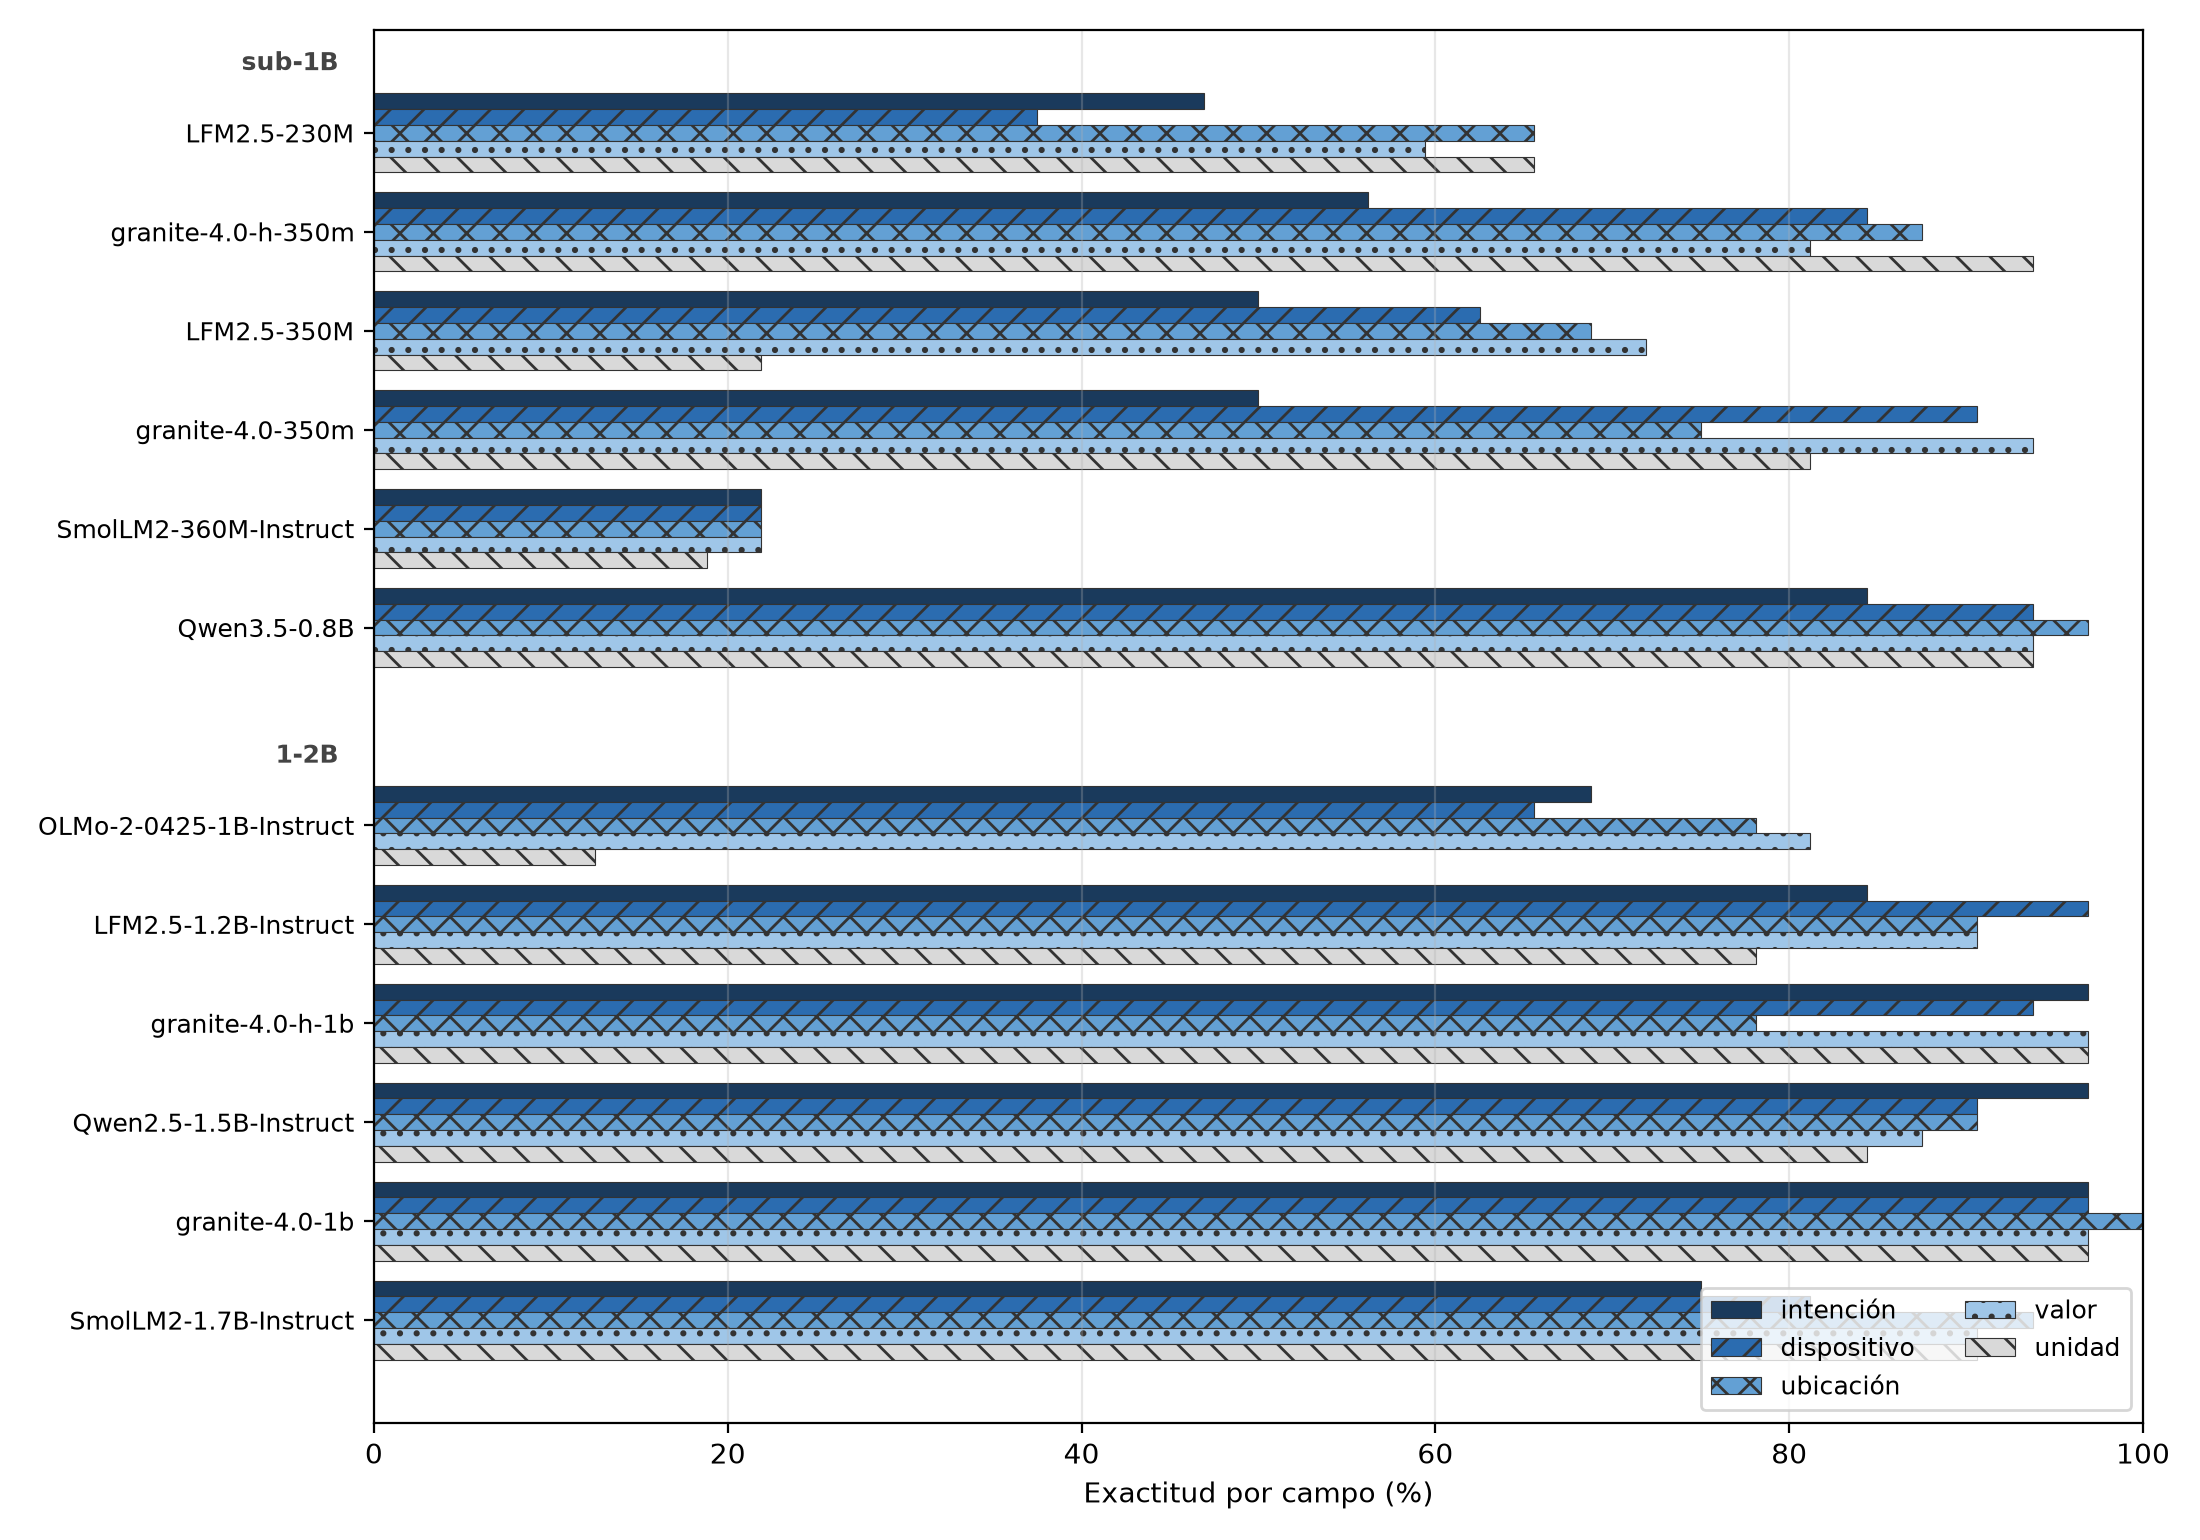
\includegraphics[width=\textwidth]{figuras/fig2_exactitud_por_campo_2026.png}
\caption{Exactitud por campo del esquema de salida (intent, dispositivo,
ubicación, valor, unidad), por modelo, agrupados por tamaño.}
\label{fig:campos}
\end{figure}

La Figura \ref{fig:campos} descompone la exactitud por cada uno de los cinco
campos del esquema de salida. Promediando sobre los doce modelos, el campo
\texttt{intent} y el campo \texttt{unidad} son los que concentran, en
promedio, la mayor tasa de error, mientras que \texttt{valor} y
\texttt{ubicacion} son los campos que los modelos resuelven de forma más
consistente. El campo \texttt{unidad} en particular muestra el rango más
amplio entre modelos: hay modelos que lo resuelven casi siempre y otros para
los que es, junto con \texttt{intent}, el campo menos confiable, lo que
sugiere que gran parte del error de exactitud estricta no proviene de una
confusión de intención grave sino de detalles de menor jerarquía semántica
del esquema (qué unidad o qué valor acompaña a un ajuste correctamente
identificado).

\subsection{Exactitud por categoría lingüística}

\begin{table}[htbp]
\centering
\caption{Exactitud estricta por categoría lingüística}
\label{tab:categorias}
\resizebox{\textwidth}{!}{%
\begin{tabular}{lrrrrrrrrrrrr}
\toprule
Categoría (n) & LFM2.5-230M & granite-4.0-h-350m & LFM2.5-350M & granite-4.0-350m & SmolLM2-360M-Instruct & Qwen3.5-0.8B & OLMo-2-0425-1B-Instruct & LFM2.5-1.2B-Instruct & granite-4.0-h-1b & Qwen2.5-1.5B-Instruct & granite-4.0-1b & SmolLM2-1.7B-Instruct \\
\midrule
Encendido / apagado simple (15) & 6.7 & 6.7 & 0.0 & 20.0 & 6.7 & 60.0 & 0.0 & 46.7 & 60.0 & 60.0 & 86.7 & 33.3 \\
Ajuste con valor numérico (14) & 7.1 & 78.6 & 0.0 & 35.7 & 7.1 & 92.9 & 7.1 & 71.4 & 92.9 & 78.6 & 100.0 & 71.4 \\
Ajuste relativo / cualitativo (3) & 0.0 & 33.3 & 0.0 & 33.3 & 33.3 & 66.7 & 0.0 & 33.3 & 33.3 & 33.3 & 66.7 & 33.3 \\
\bottomrule
\end{tabular}
}
\end{table}


Las categorías lingüísticas de la Tabla \ref{tab:categorias} no las asignó un
anotador humano, como en la ronda inicial de este experimento, sino el juez
automático descripto en la Sección \ref{sec:dos-etapas}, sobre el mismo
vocabulario cerrado de seis categorías del dataset original. La comparación
contra la distribución de esa ronda inicial (8/8/6/4/3/3 sobre las seis
categorías) revela una diferencia que no conviene ocultar: el juez automático, en esta corrida, sólo utilizó
tres de las seis categorías cerradas —\emph{encendido/apagado simple}
(15 comandos), \emph{ajuste con valor numérico} (14) y \emph{ajuste relativo o
cualitativo} (3)— y ninguno de los 32 comandos quedó clasificado en
\emph{múltiples dispositivos}, \emph{consulta de estado} ni \emph{negación o
contexto conversacional}. Una inspección de las asignaciones muestra el patrón
del colapso: comandos que preguntan por un estado (``¿Está prendida la luz del
living?''), que niegan una acción previa (``No dejes prendida la luz de la
cocina, apagala'') o que involucran varios dispositivos a la vez (``Apagá
todas las luces de la casa'') quedaron plegados dentro de
\emph{encendido/apagado simple} o de \emph{ajuste relativo o cualitativo} en
lugar de formar sus propias categorías. Esto no afecta la exactitud estricta
ni laxa, que se calculan por comando y no dependen de la categoría asignada,
pero sí limita el valor de la Tabla \ref{tab:categorias} como desagregación
lingüística fina en esta corrida, y se retoma como una limitación de la
asignación automática de categoría en la Sección 6.

\subsection{Análisis automático de errores}
\label{sec:analisis-errores}

\begin{table}[htbp]
\centering
\caption{Distribución de errores por categoría de la taxonomía}
\label{tab:taxonomia}
\resizebox{\textwidth}{!}{%
\begin{tabular}{lrrrrrrrrrrrr}
\toprule
Categoría de error & LFM2.5-230M & LFM2.5-350M & granite-4.0-350m & granite-4.0-h-350m & Qwen3.5-0.8B & SmolLM2-360M-Instruct & LFM2.5-1.2B-Instruct & granite-4.0-1b & granite-4.0-h-1b & OLMo-2-0425-1B-Instruct & SmolLM2-1.7B-Instruct & Qwen2.5-1.5B-Instruct \\
\midrule
Total de respuestas incorrectas & 30 & 32 & 23 & 19 & 8 & 29 & 14 & 3 & 9 & 31 & 16 & 11 \\
Confusión de intención & 0 & 0 & 3 & 0 & 1 & 0 & 2 & 0 & 0 & 0 & 0 & 0 \\
Confusión de dispositivo & 20 & 20 & 9 & 9 & 4 & 2 & 3 & 0 & 1 & 19 & 5 & 1 \\
Confusión de ubicación & 4 & 5 & 0 & 0 & 0 & 0 & 0 & 0 & 0 & 3 & 0 & 1 \\
Alucinación de valor/unidad & 0 & 0 & 0 & 0 & 0 & 0 & 0 & 0 & 0 & 0 & 0 & 0 \\
Valor numérico incorrecto & 0 & 0 & 0 & 0 & 0 & 0 & 0 & 0 & 0 & 1 & 0 & 0 \\
Sin error semántico & 1 & 1 & 5 & 3 & 0 & 1 & 2 & 1 & 7 & 2 & 5 & 2 \\
Uso de sinónimos & 8 & 11 & 6 & 7 & 3 & 26 & 7 & 2 & 1 & 9 & 6 & 7 \\
\bottomrule
\end{tabular}
}
\end{table}


Esta subsección reemplaza la revisión manual de respuestas incorrectas de la
ronda inicial de este experimento por una clasificación completamente
automática. El juez es el
modelo seleccionado por la regla congelada de la Sección \ref{sec:dos-etapas}
—mayor exactitud estricta de la etapa 1, empate hacia el modelo de mayor
tamaño—, que en este barrido es \texttt{granite-4.0-1b}, con \textbf{90,6\%}
de exactitud estricta en la etapa 1 (el mismo valor que su exactitud estricta
final, porque no cambia entre etapas). Cada una de las 225 respuestas con
\texttt{match\_exact = False} se clasificó en un subconjunto no vacío de las
\textbf{siete} etiquetas de la Tabla \ref{tab:taxonomia} —las cinco heredadas
de la ronda inicial de este experimento, con \emph{alucinación de valor/unidad} y \emph{valor
numérico incorrecto} ya separadas en dos etiquetas distintas en vez de
fusionadas en una, más \emph{sin error semántico} y \emph{uso de sinónimos},
que son precisamente las que definen la exactitud laxa—. Ninguna de las 225
respuestas clasificadas, ni ninguna de las 32 asignaciones de categoría
lingüística de la Sección 4.3, quedó con \texttt{juez\_parse\_ok = False}: el
juez no necesitó ningún reintento ni ninguna etiqueta de respaldo en esta
corrida.

La métrica laxa rescató, en conjunto, \textbf{123} de las 225 respuestas
incorrectas bajo el protocolo estricto (etiquetadas \texttt{sin\_error\_semantico}
o \texttt{uso\_de\_sinonimos}), es decir algo menos de un tercio de las 384
respuestas totales del barrido. Un ejemplo puntual, relevante para la Sección
5: de las 30 respuestas incorrectas de \texttt{LFM2.5-230M}, \textbf{9} son
\texttt{uso\_de\_sinonimos} o \texttt{sin\_error\_semantico} — casi un tercio
de sus errores estrictos no son errores de contenido sino de vocabulario.

La Tabla \ref{tab:taxonomia} por sí sola no distingue, sin embargo, entre dos
formas muy distintas de tener exactitud estricta cercana a cero, y esa
distinción es un requisito de este trabajo: un \texttt{json\_valido} alto
junto a una exactitud casi nula indica que el modelo emite el formato
correctamente y se equivoca en el contenido —un fallo semántico genuino, y un
resultado en sí mismo—, mientras que un \texttt{json\_valido} bajo junto a una
exactitud casi nula indica que el modelo ni siquiera logra emitir el formato
—un artefacto de parseo, no una incapacidad semántica—. Sobre la Tabla
\ref{tab:globales}: \texttt{LFM2.5-350M} tiene 0,0\% de exactitud estricta con
\textbf{100\%} de JSON válido, y \texttt{OLMo-2-0425-1B-Instruct} tiene 3,1\%
de exactitud estricta con también \textbf{100\%} de JSON válido — ambos son,
por lo tanto, fallos semánticos genuinos. \texttt{SmolLM2-360M-Instruct}, en
cambio, tiene 9,4\% de exactitud estricta pero sólo \textbf{25\%} de JSON
válido: su exactitud casi nula es, en buena medida, un artefacto de formato, y
tratarla como incapacidad semántica contaminaría la conclusión. Por esta razón
la afirmación de ``100\% de JSON válido'' de la ronda inicial de este
experimento no puede repetirse sin matices en este trabajo: con el roster
de doce modelos la validez de formato
no es universal (25\% en \texttt{SmolLM2-360M-Instruct}, 87,5\% en
\texttt{LFM2.5-230M}, y 100\% en los nueve modelos restantes).

Esta distinción tiene además una consecuencia directa sobre la confiabilidad
de la propia métrica laxa, que conviene declarar aquí explícitamente en vez de
como una nota al pie: la métrica laxa es poco confiable exactamente donde la
validez de formato es débil. El campo \texttt{laxo\_json\_invalido\_n} —el
número de respuestas que el juez etiquetó \texttt{sin\_error\_semantico} o
\texttt{uso\_de\_sinonimos} (y que por lo tanto cuentan para la exactitud laxa)
pese a que su JSON no era válido— es \textbf{24} para
\texttt{SmolLM2-360M-Instruct}, sobre apenas \textbf{27} respuestas rescatadas
en total por la métrica laxa para ese modelo: es decir que 24 de esas 27
respuestas ``semánticamente equivalentes'' tenían JSON inválido, y el juez las
acreditó de todos modos. Su exactitud laxa de 93,8\% es, en consecuencia, un
artefacto de la fragilidad de formato de este modelo, no evidencia de
competencia semántica. El mismo campo vale \textbf{4} para
\texttt{LFM2.5-230M} (sobre 9 respuestas rescatadas) y \textbf{0} para los diez
modelos restantes. Esta amenaza a la confiabilidad de la métrica laxa se
retoma en la Sección 6.

\section{Discusión}

\textbf{La brecha entre exactitud estricta y laxa} mide cuánto penaliza la
coincidencia textual exacta a respuestas que un juez semántico considera
equivalentes, y la taxonomía la descompone en dos causas: ausencia de error
semántico, y sustitución de un valor del vocabulario cerrado por un sinónimo.

\textbf{Endurecer el prompt no elimina el problema.} Aunque el prompt declara
que un sinónimo de un valor categórico cerrado es una violación de formato
(Sección \ref{sec:prompting}), \texttt{uso\_de\_sinonimos} aparece en
prácticamente todos los modelos: copiar textualmente un token de una lista
cerrada exige un tipo de obediencia distinto del que exige acertar el
contenido, y varios modelos con buena exactitud de campo prefieren la forma
natural (``tele'') sobre la literal exigida (``tv''). El caso extremo es
\texttt{SmolLM2-360M-Instruct}, cuyas respuestas incorrectas se explican casi
por completo por esta única causa (Tabla \ref{tab:taxonomia}).

\textbf{Tamaño, arquitectura y generación.} Que \texttt{Qwen3.5-0.8B} supere
a cuatro de los seis modelos del tier superior con menos de mil millones de
parámetros muestra que el desempeño no depende sólo del conteo de parámetros,
y los +25,0 puntos de \texttt{granite-4.0-1b} sobre el mejor modelo de la
generación anterior cuantifican el desplazamiento de lo factible en el rango
sub-2B.

\textbf{Penalización de latencia de la atención híbrida.}
\label{sec:discusion-latencia-hibrida}
\texttt{granite-4.0-h-350m} tarda \textbf{56,45} segundos por comando frente
a los \textbf{13,77} de la variante densa \texttt{granite-4.0-350m}
(\textbf{$\times$4,10}), y \texttt{granite-4.0-h-1b} \textbf{123,15} frente a
los \textbf{42,78} de \texttt{granite-4.0-1b} (\textbf{$\times$2,88}). Que se
reproduzca en \textbf{ambos} pares de tamaño, con la misma familia y el mismo
protocolo, indica un efecto arquitectónico y no un artefacto puntual. Las
variantes híbridas se promocionan por su complejidad sub-cuadrática en la
longitud de secuencia, beneficio que se materializa en secuencias largas;
aquí los prompts son \textbf{cortos} y la ejecución es sobre \textbf{CPU}, de
modo que ese beneficio asintótico no llega a manifestarse mientras que la
sobrecarga \textbf{constante} de gestionar dos tipos de caché —atención
estándar y estado lineal/recurrente— se paga en cada comando y domina el
tiempo total. \textbf{A igual cantidad de parámetros, la variante densa es
preferible en CPU para prompts cortos.}

\textbf{Viabilidad práctica.} Los 42,78 segundos por comando del modelo más
exacto son incompatibles con una interacción de voz en tiempo real, aunque
aceptables para automatización diferida; entre los sub-1B,
\texttt{Qwen3.5-0.8B} combina 75,0\% de exactitud estricta con 18,17
segundos, el compromiso más equilibrado del roster.

\section{Amenazas a la validez}

\textbf{Validez de constructo.} La métrica principal (exactitud estricta)
exige coincidencia textual con el ground truth bajo un protocolo que declara
explícitamente los sinónimos de valores categóricos cerrados como violación de
formato (Sección \ref{sec:prompting}). Esta amenaza ya no es sólo una
advertencia sin cuantificar, como en la ronda inicial de este experimento: queda
\textbf{resuelta parcialmente} por la exactitud laxa y por la taxonomía de
errores de la Sección \ref{sec:analisis-errores}, que separan explícitamente
cuánta exactitud estricta perdida corresponde a \texttt{uso\_de\_sinonimos} o
a \texttt{sin\_error\_semantico} en lugar de a un error de contenido real. La
brecha sigue siendo una cota superior semántica, no una medición
independiente con un evaluador humano, y la Sección 4.4 mostró que esta
métrica laxa es a su vez poco confiable donde la validez de formato es débil:
24 de las 27 respuestas que la métrica laxa acreditó a
\texttt{SmolLM2-360M-Instruct} tenían JSON inválido (ver más abajo, amenaza de
validez interna sobre el sesgo del juez y la fragilidad de
\texttt{SmolLM2-360M-Instruct}).

\textbf{Validez interna.}

\emph{Sesgo de auto-favorecimiento del juez.} El juez de la etapa 2 es
\texttt{granite-4.0-1b}, seleccionado por la regla congelada de mayor
exactitud estricta en la etapa 1 (Sección \ref{sec:dos-etapas}), y ese mismo
modelo es uno de los doce evaluados: \textbf{juzga también sus propias
respuestas de la etapa 1}. Un juez basado en LLM puede favorecer respuestas
generadas por sí mismo o por modelos de su misma familia
\cite{zheng2023judging}, y en este diseño esa posibilidad no está controlada
ni por un juez externo ni por un segundo evaluador independiente. El riesgo es
mayor todavía porque, al ser el modelo con mayor exactitud estricta de la
etapa 1, \texttt{granite-4.0-1b} es también el modelo con \textbf{menos}
respuestas incorrectas en juego (apenas 3 de 32, Tabla \ref{tab:taxonomia}):
tiene la menor cantidad relativa de casos propios para favorecer, lo que
acota — sin eliminar — el margen concreto de ese sesgo sobre el resultado
agregado. Además, es un modelo de menos de 2 mil millones de parámetros
adjudicando equivalencia semántica en lenguaje natural, una tarea de juicio
más exigente que la clasificación de campos estructurados, con la capacidad
limitada que ese tamaño implica; los 0 casos de \texttt{juez\_parse\_ok = False}
reportados en la Sección \ref{sec:analisis-errores} indican que el juez sí
logró producir salidas parseables de forma consistente, pero no dicen nada
sobre la calidad de su criterio semántico. Mitigar esta amenaza en trabajo
futuro requeriría un juez externo de mayor escala, no perteneciente al roster
evaluado, o una validación humana sobre una muestra de sus adjudicaciones.
Como contrapeso, la adjudicación es \textbf{reproducible por diseño}: ambas
etapas corren con decodificación greedy (\texttt{do\_sample=False},
temperatura 0), de modo que, dado el mismo modelo de entrada, cualquiera puede
re-ejecutar el juicio y obtener exactamente el mismo resultado.

\emph{Versiones divergentes de la librería de inferencia como confusor de
latencia.} Los doce modelos del roster activo corren bajo \textbf{dos grupos
de versión} de \texttt{transformers}, mutuamente excluyentes (Tabla
\ref{tab:versiones}): el grupo A resuelve a la versión 4.57.6, con
\textbf{9} modelos, y el grupo B resuelve a la versión 5.14.1, con los
\textbf{3} restantes. Esto es un confusor conocido para cualquier comparación
de \textbf{latencia} entre un modelo del grupo A y uno del grupo B: parte de
la diferencia observada puede deberse a la versión de la librería y no al
modelo en sí. Cada grupo está forzado por evidencia empírica propia, no por
preferencia de diseño: \texttt{granite-4.0-350m} necesita el grupo A porque
falla bajo 5.14.1; \texttt{LFM2.5-230M}, \texttt{LFM2.5-350M} y
\texttt{Qwen3.5-0.8B} necesitan el grupo B porque fallan bajo 4.57.6. La
evidencia más nítida de que el confusor no es un artefacto teórico es que el
grupo B resuelve exactamente a la versión (5.14.1) que rompe al modelo que
fuerza el grupo A: ninguna versión mayor única cubre el roster completo. No
se repite aquí la premisa, ya descartada en este mismo trabajo, de que una
única versión mayor de \texttt{transformers} elimina este confusor: la
evidencia de ambos grupos activos la refuta en las dos direcciones.

\emph{Topología de procesadores no observable.} La Sección
\ref{sec:entorno-repro} estableció que la configuración de Docker de esta
máquina expone únicamente 2 procesadores lógicos a los contenedores, y que
\texttt{-{}-cpuset-cpus=0-1} fija ese mismo par en las doce corridas y en la
del juez. Qué relación guardan esos 2 procesadores lógicos con los núcleos
físicos del host —hermanos de un mismo núcleo por \emph{hyperthreading}
(SMT), lo que introduciría contención adicional entre ellos, o dos núcleos
físicos distintos, sin esa contención— la decide el hipervisor de esa
configuración de Docker, y esta amenaza a la validez no puede resolverse
observando desde adentro del contenedor: la topología efectiva no quedó bajo
control de este experimento. Esto afecta por igual a los doce modelos —todos
corrieron bajo el mismo tope, de a uno por vez—, así que no introduce un
sesgo relativo entre ellos, pero sí implica que los valores absolutos de
latencia reportados pueden estar inflados por contención respecto de lo que
esta misma máquina lograría con dos núcleos físicos completos, y no deben
leerse como la mejor latencia alcanzable en este hardware. Los cocientes de
latencia entre variantes híbridas y densas de la Sección
\ref{sec:discusion-latencia-hibrida} (\texttt{$\times$4,10} y
\texttt{$\times$2,88}) son robustos a esta amenaza precisamente porque
comparan pares de modelos medidos bajo la misma topología, cualquiera haya
sido.

\textbf{Validez externa.}

Se conservan además las amenazas de validez externa de la ronda inicial de
este experimento: el dataset de evaluación es chico y desbalanceado (32
comandos, entre 3 y 8 por categoría lingüística), se usó un único prompt sin
optimización específica por modelo, la entrada fue siempre texto limpio sin
ruido de reconocimiento de voz (ASR), y sólo se cubrió una variante
dialectal (español rioplatense).

\textbf{Validez de conclusión.} Con entre 3 y 8 comandos por categoría, las
diferencias porcentuales entre modelos de la Tabla \ref{tab:categorias} y de
la Tabla \ref{tab:globales} son indicativas, no estadísticamente
significativas en sentido formal — la misma limitación de la ronda inicial
de este experimento, que este trabajo no resuelve. Todas las corridas del
barrido principal (Sección \ref{sec:entorno-repro}) se ejecutaron en una
\textbf{única máquina}, de forma estrictamente secuencial y con
procesadores fijos, para que la latencia fuera comparable entre modelos;
las corridas de control, en cambio, compartieron la máquina con trabajo
concurrente del orquestador y por eso se excluyen explícitamente de
cualquier afirmación de latencia de este trabajo, quedando limitadas a la
justificación metodológica de la Sección \ref{sec:entorno-repro}. Por último,
\texttt{attn\_implementation} y la \texttt{revision} exacta de cada modelo de
HuggingFace quedaron, también en este trabajo, \textbf{sin pinnear}: cada
corrida usó lo que \texttt{transformers} resolviera por defecto en el momento
de ejecutarse, y ningún registro deja constancia de qué implementación de
atención ni qué revisión de pesos se usó exactamente. Pinnear ambos valores
ahora exigiría re-correr el barrido completo para que la comparación siguiera
siendo de igual a igual, lo que explícitamente no se consideró que valiera la
pena frente al beneficio; se documenta aquí como limitación conocida y no como
un defecto corregido.

\section{Conclusiones y trabajo futuro}

Este trabajo evaluó automáticamente doce SLMs abiertos de menos de 2 mil
millones de parámetros interpretando comandos de domótica en español
rioplatense, con un procedimiento de dos etapas y decodificación determinista
que reemplaza toda anotación manual: es reproducible por construcción y
escala a conjuntos mucho mayores sin que el costo de anotación crezca. Bajo
el mismo prompt, \texttt{granite-4.0-1b} alcanza 90,6\% de exactitud
estricta, 25,0 puntos porcentuales por encima de
\texttt{Qwen2.5-1.5B-Instruct} (65,6\%), incorporado deliberadamente como
representante de la generación anterior y medido bajo el mismo protocolo.

Como trabajo futuro se plantea incorporar un juez externo de mayor escala o
validación humana sobre una muestra; ampliar y balancear el dataset,
incluyendo voz real transcrita por ASR; cubrir otras variantes dialectales; y
repetir el barrido sobre un host con más de 2 procesadores lógicos.

\section*{Declaración sobre el uso de IA}

Se utilizaron herramientas de inteligencia artificial generativa en el diseño
y la curación del dataset y de las taxonomías cerradas, en el desarrollo del
código de evaluación, en la redacción y edición del manuscrito, y en la
generación de las figuras y tablas de resultados. A esos cuatro roles se
agrega un quinto, de naturaleza distinta: un modelo de lenguaje cumple un rol
\textbf{metodológico} como juez automático (Sección \ref{sec:dos-etapas}).
Ese rol no es asistencia editorial sino parte del método experimental: sus
salidas son datos del estudio, sujetos a las mismas amenazas a la validez que
cualquier otra medición. Los resultados corresponden a la ejecución real de
los modelos evaluados y a la adjudicación real del juez. Los autores
revisaron, validaron y son responsables del contenido, el análisis y las
conclusiones, en línea con marcos de buenas prácticas propuestos
recientemente para la divulgación del uso de agentes de IA en la
investigación académica \cite{torassa2025etica}.


\bibliographystyle{splncs03}
\bibliography{refs}

\end{document}
